\documentclass[]{article}
\usepackage{lmodern}
\usepackage{amssymb,amsmath}
\usepackage{ifxetex,ifluatex}
\usepackage{fixltx2e} % provides \textsubscript
\ifnum 0\ifxetex 1\fi\ifluatex 1\fi=0 % if pdftex
  \usepackage[T1]{fontenc}
  \usepackage[utf8]{inputenc}
\else % if luatex or xelatex
  \ifxetex
    \usepackage{mathspec}
  \else
    \usepackage{fontspec}
  \fi
  \defaultfontfeatures{Ligatures=TeX,Scale=MatchLowercase}
\fi
% use upquote if available, for straight quotes in verbatim environments
\IfFileExists{upquote.sty}{\usepackage{upquote}}{}
% use microtype if available
\IfFileExists{microtype.sty}{%
\usepackage{microtype}
\UseMicrotypeSet[protrusion]{basicmath} % disable protrusion for tt fonts
}{}
\usepackage[margin=1in]{geometry}
\usepackage{hyperref}
\hypersetup{unicode=true,
            pdftitle={Discussion\_week5},
            pdfauthor={Salma Elshahawy},
            pdfborder={0 0 0},
            breaklinks=true}
\urlstyle{same}  % don't use monospace font for urls
\usepackage{color}
\usepackage{fancyvrb}
\newcommand{\VerbBar}{|}
\newcommand{\VERB}{\Verb[commandchars=\\\{\}]}
\DefineVerbatimEnvironment{Highlighting}{Verbatim}{commandchars=\\\{\}}
% Add ',fontsize=\small' for more characters per line
\usepackage{framed}
\definecolor{shadecolor}{RGB}{248,248,248}
\newenvironment{Shaded}{\begin{snugshade}}{\end{snugshade}}
\newcommand{\AlertTok}[1]{\textcolor[rgb]{0.94,0.16,0.16}{#1}}
\newcommand{\AnnotationTok}[1]{\textcolor[rgb]{0.56,0.35,0.01}{\textbf{\textit{#1}}}}
\newcommand{\AttributeTok}[1]{\textcolor[rgb]{0.77,0.63,0.00}{#1}}
\newcommand{\BaseNTok}[1]{\textcolor[rgb]{0.00,0.00,0.81}{#1}}
\newcommand{\BuiltInTok}[1]{#1}
\newcommand{\CharTok}[1]{\textcolor[rgb]{0.31,0.60,0.02}{#1}}
\newcommand{\CommentTok}[1]{\textcolor[rgb]{0.56,0.35,0.01}{\textit{#1}}}
\newcommand{\CommentVarTok}[1]{\textcolor[rgb]{0.56,0.35,0.01}{\textbf{\textit{#1}}}}
\newcommand{\ConstantTok}[1]{\textcolor[rgb]{0.00,0.00,0.00}{#1}}
\newcommand{\ControlFlowTok}[1]{\textcolor[rgb]{0.13,0.29,0.53}{\textbf{#1}}}
\newcommand{\DataTypeTok}[1]{\textcolor[rgb]{0.13,0.29,0.53}{#1}}
\newcommand{\DecValTok}[1]{\textcolor[rgb]{0.00,0.00,0.81}{#1}}
\newcommand{\DocumentationTok}[1]{\textcolor[rgb]{0.56,0.35,0.01}{\textbf{\textit{#1}}}}
\newcommand{\ErrorTok}[1]{\textcolor[rgb]{0.64,0.00,0.00}{\textbf{#1}}}
\newcommand{\ExtensionTok}[1]{#1}
\newcommand{\FloatTok}[1]{\textcolor[rgb]{0.00,0.00,0.81}{#1}}
\newcommand{\FunctionTok}[1]{\textcolor[rgb]{0.00,0.00,0.00}{#1}}
\newcommand{\ImportTok}[1]{#1}
\newcommand{\InformationTok}[1]{\textcolor[rgb]{0.56,0.35,0.01}{\textbf{\textit{#1}}}}
\newcommand{\KeywordTok}[1]{\textcolor[rgb]{0.13,0.29,0.53}{\textbf{#1}}}
\newcommand{\NormalTok}[1]{#1}
\newcommand{\OperatorTok}[1]{\textcolor[rgb]{0.81,0.36,0.00}{\textbf{#1}}}
\newcommand{\OtherTok}[1]{\textcolor[rgb]{0.56,0.35,0.01}{#1}}
\newcommand{\PreprocessorTok}[1]{\textcolor[rgb]{0.56,0.35,0.01}{\textit{#1}}}
\newcommand{\RegionMarkerTok}[1]{#1}
\newcommand{\SpecialCharTok}[1]{\textcolor[rgb]{0.00,0.00,0.00}{#1}}
\newcommand{\SpecialStringTok}[1]{\textcolor[rgb]{0.31,0.60,0.02}{#1}}
\newcommand{\StringTok}[1]{\textcolor[rgb]{0.31,0.60,0.02}{#1}}
\newcommand{\VariableTok}[1]{\textcolor[rgb]{0.00,0.00,0.00}{#1}}
\newcommand{\VerbatimStringTok}[1]{\textcolor[rgb]{0.31,0.60,0.02}{#1}}
\newcommand{\WarningTok}[1]{\textcolor[rgb]{0.56,0.35,0.01}{\textbf{\textit{#1}}}}
\usepackage{graphicx,grffile}
\makeatletter
\def\maxwidth{\ifdim\Gin@nat@width>\linewidth\linewidth\else\Gin@nat@width\fi}
\def\maxheight{\ifdim\Gin@nat@height>\textheight\textheight\else\Gin@nat@height\fi}
\makeatother
% Scale images if necessary, so that they will not overflow the page
% margins by default, and it is still possible to overwrite the defaults
% using explicit options in \includegraphics[width, height, ...]{}
\setkeys{Gin}{width=\maxwidth,height=\maxheight,keepaspectratio}
\IfFileExists{parskip.sty}{%
\usepackage{parskip}
}{% else
\setlength{\parindent}{0pt}
\setlength{\parskip}{6pt plus 2pt minus 1pt}
}
\setlength{\emergencystretch}{3em}  % prevent overfull lines
\providecommand{\tightlist}{%
  \setlength{\itemsep}{0pt}\setlength{\parskip}{0pt}}
\setcounter{secnumdepth}{0}
% Redefines (sub)paragraphs to behave more like sections
\ifx\paragraph\undefined\else
\let\oldparagraph\paragraph
\renewcommand{\paragraph}[1]{\oldparagraph{#1}\mbox{}}
\fi
\ifx\subparagraph\undefined\else
\let\oldsubparagraph\subparagraph
\renewcommand{\subparagraph}[1]{\oldsubparagraph{#1}\mbox{}}
\fi

%%% Use protect on footnotes to avoid problems with footnotes in titles
\let\rmarkdownfootnote\footnote%
\def\footnote{\protect\rmarkdownfootnote}

%%% Change title format to be more compact
\usepackage{titling}

% Create subtitle command for use in maketitle
\providecommand{\subtitle}[1]{
  \posttitle{
    \begin{center}\large#1\end{center}
    }
}

\setlength{\droptitle}{-2em}

  \title{Discussion\_week5}
    \pretitle{\vspace{\droptitle}\centering\huge}
  \posttitle{\par}
    \author{Salma Elshahawy}
    \preauthor{\centering\large\emph}
  \postauthor{\par}
      \predate{\centering\large\emph}
  \postdate{\par}
    \date{2/25/2020}

\usepackage{geometry}

\begin{document}
\maketitle

Mathematicians have been known to get some of the best ideas while
sitting in a cafe, riding on a bus, or strolling in the park. In the
early 1900s the famous mathematician George P ́olya lived in a hotel near
the woods in Zurich. He liked to walk in the woods and think about
mathematics. P ́olya describes the following incident:

\begin{figure}
\centering
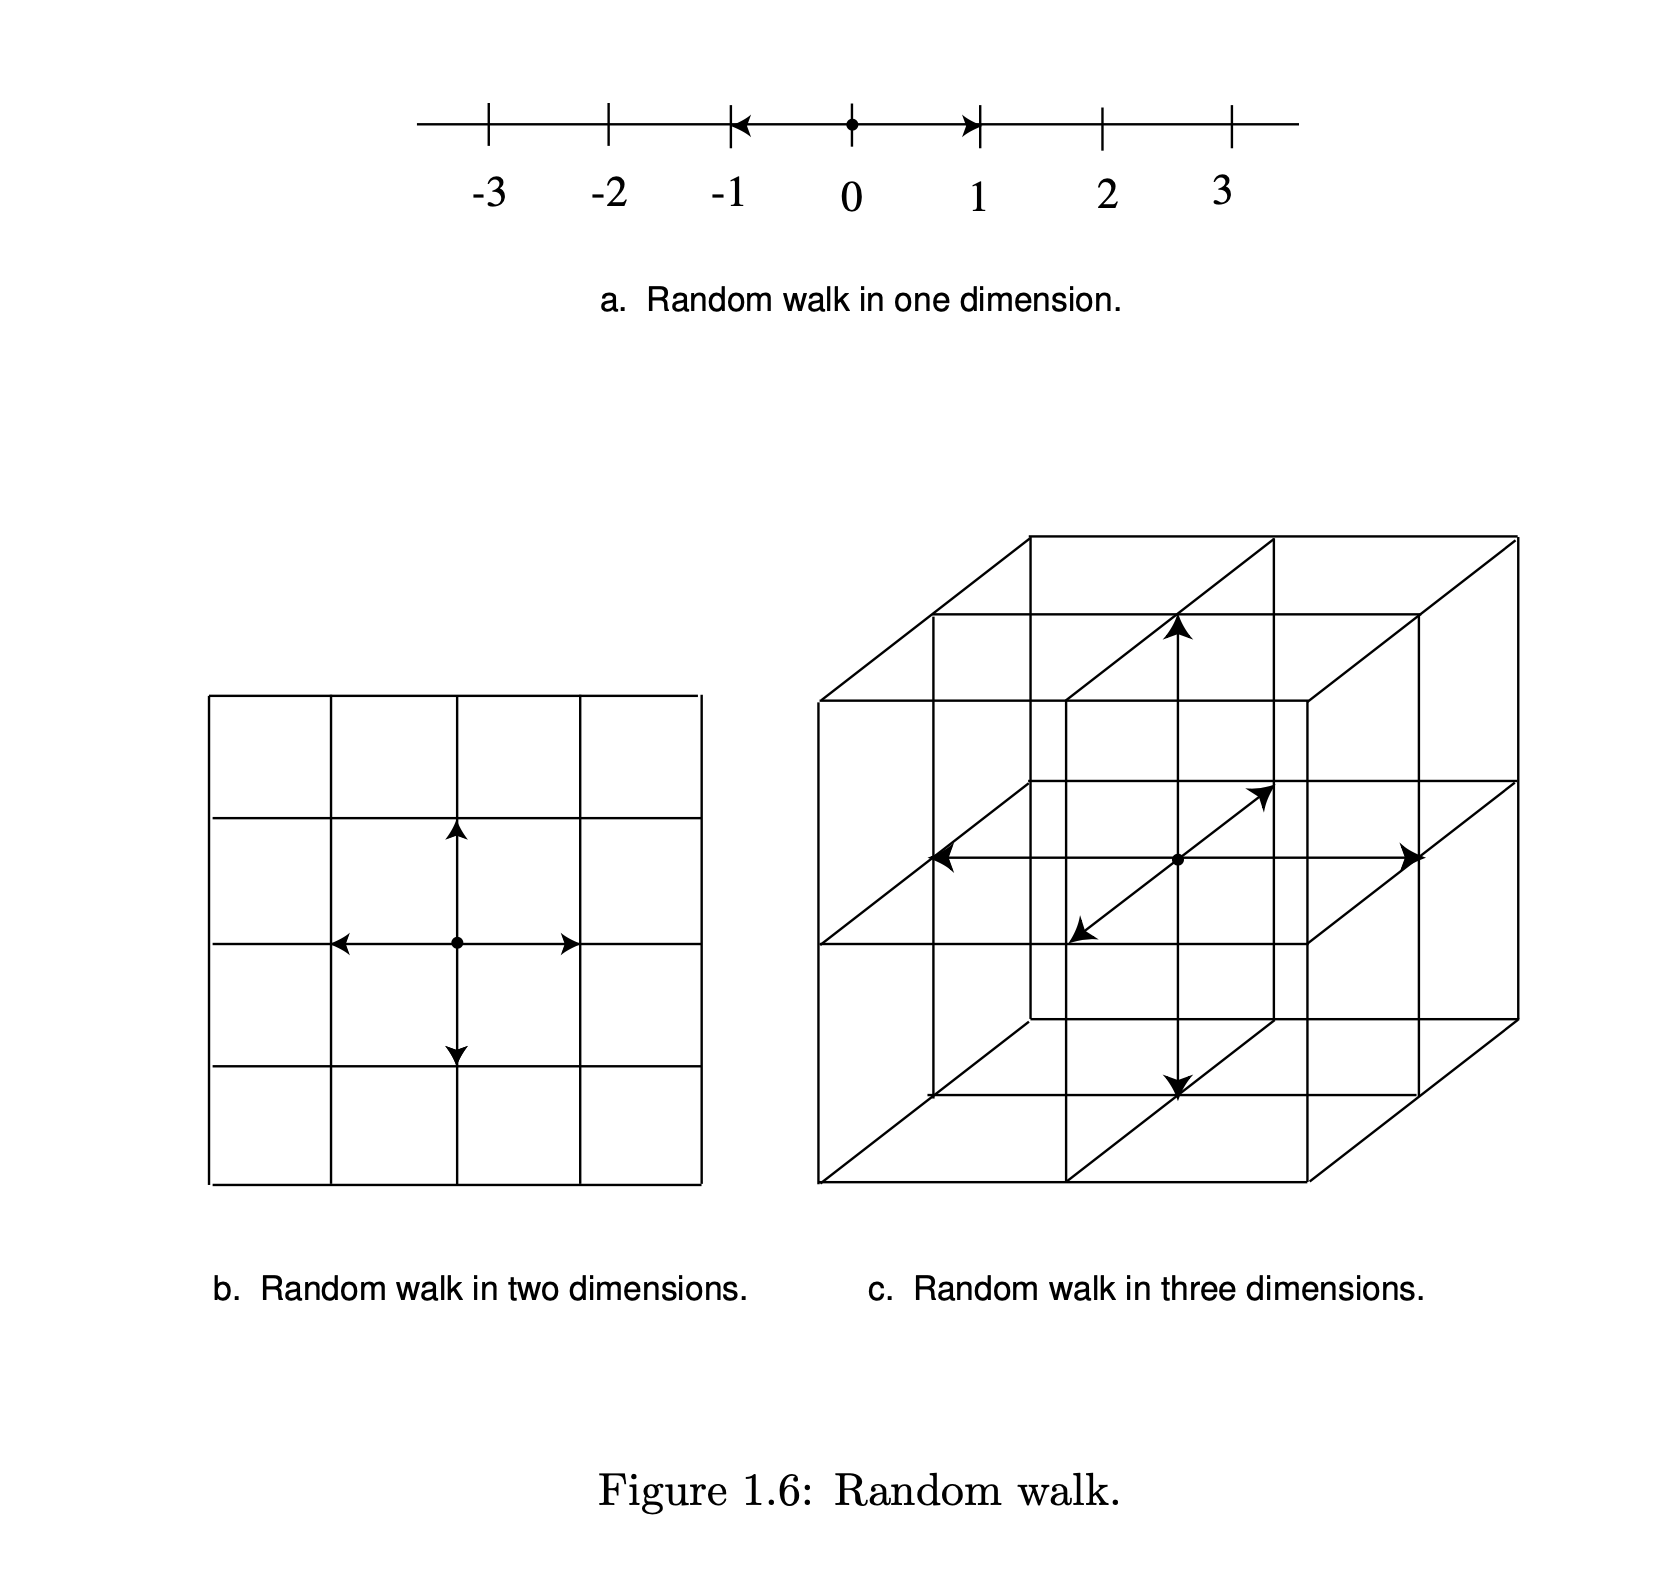
\includegraphics{/Users/salmaelshahawy/Desktop/MSDS_SP2020/Spring2020/computational_mod_605/Week_5/random_walk.png}
\caption{random\_walk}
\end{figure}

At the hotel there lived also some students with whom I usually took my
meals and had friendly relations. On a certain day one of them expected
the visit of his fianćee, what (sic) I knew, but I did not foresee that
he and his fianc ́ee would also set out for a stroll in the woods, and
then suddenly I met them there. And then I met them the same morning
repeatedly, I don't remember how many times, but certainly much too
often and I felt embarrassed: It looked as if I was snooping around
which was, I assure you, not the case. This set him to thinking about
whether random walkers were destined to meet.P ́olya considered random
walkers in one, two, and three dimensions. In one dimension, he
envisioned the walker on a very long street. At each intersec- tion the
walker flips a fair coin to decide which direction to walk next (see
Figure 1.6a). In two dimensions, the walker is walking on a grid of
streets, and at each intersection he chooses one of the four possible
directions with equal probability (see Figure). In three dimensions (we
might better speak of a random climber), the walker moves on a
three-dimensional grid, and at each intersection there are now six
different directions that the walker may choose, each with equal
probability

Write a program to simulate a random walk in one dimension starting at
0. Have your program print out the lengths of the times between returns
to the starting point (returns to 0). See if you can guess from this
simulation the answer to the following question: Will the walker always
return to his starting point eventually or might he drift away forever?

\begin{Shaded}
\begin{Highlighting}[]
\CommentTok{# a random walk on the integers is a sequence X0, X1,...with X0 = 0}
\CommentTok{# and Xi = Xi-1 + Di where Di is independent, equal to +1 with probability p, and otherwise -1}
\NormalTok{Random_walk <-}\StringTok{ }\ControlFlowTok{function}\NormalTok{(x, }\DataTypeTok{size=}\DecValTok{10000}\NormalTok{)\{}
  \CommentTok{# This function is used to generate random walk}
  \CommentTok{# x : the point that you want to reach}
  \CommentTok{# size : how large the sample size you want to have at one time. This has default value 1000}
  
  \CommentTok{# If the point is too large, try to choose larger sample size to shorten the time.}
  \KeywordTok{set.seed}\NormalTok{(}\DecValTok{123}\NormalTok{) }\CommentTok{# To generate same result every time}
\NormalTok{  previous <-}\StringTok{ }\DecValTok{0}
\NormalTok{  positions <-}\StringTok{ }\DecValTok{0}
\NormalTok{  s <-}\StringTok{ }\DecValTok{1} 
\NormalTok{  final <-}\StringTok{ }\DecValTok{0}
\NormalTok{  continue <-}\StringTok{ }\OtherTok{TRUE}
  \ControlFlowTok{while}\NormalTok{(continue)\{}
    \CommentTok{# generate a vector for the move T(D1,....Dsize)}
\NormalTok{    move <-}\StringTok{ }\KeywordTok{sample}\NormalTok{(}\KeywordTok{c}\NormalTok{(}\DecValTok{1}\NormalTok{,}\OperatorTok{-}\DecValTok{1}\NormalTok{), }\DataTypeTok{size =}\NormalTok{ size,}\OtherTok{TRUE}\NormalTok{)}
    \CommentTok{# Use cumsum to generate X}
\NormalTok{    previous <-}\StringTok{ }\KeywordTok{tail}\NormalTok{(final,}\DecValTok{1}\NormalTok{) }\OperatorTok{+}\StringTok{ }\KeywordTok{cumsum}\NormalTok{(move)}
      \ControlFlowTok{if}\NormalTok{(}\OperatorTok{!}\KeywordTok{is.na}\NormalTok{(}\KeywordTok{which}\NormalTok{(previous }\OperatorTok{==}\StringTok{ }\NormalTok{x)[}\DecValTok{1}\NormalTok{]))\{}
\NormalTok{        position <-}\StringTok{ }\KeywordTok{which}\NormalTok{(previous }\OperatorTok{==}\StringTok{ }\NormalTok{x)[}\DecValTok{1}\NormalTok{]}
        \KeywordTok{cat}\NormalTok{(}\StringTok{"The total steps by far is: "}\NormalTok{, position }\OperatorTok{+}\StringTok{ }\NormalTok{(s}\DecValTok{-1}\NormalTok{)}\OperatorTok{*}\NormalTok{size, }\StringTok{"}\CharTok{\textbackslash{}n}\StringTok{"}\NormalTok{)}
\NormalTok{        continue <-}\StringTok{ }\OtherTok{FALSE}
\NormalTok{      \}}\ControlFlowTok{else}\NormalTok{\{}
\NormalTok{        positions[s] <-}\StringTok{ }\NormalTok{previous[size]}
\NormalTok{        final<-}\KeywordTok{tail}\NormalTok{(positions,}\DecValTok{1}\NormalTok{)}
\NormalTok{        s <-}\StringTok{ }\NormalTok{s}\OperatorTok{+}\DecValTok{1}
\NormalTok{      \}}
\NormalTok{  \}}
\NormalTok{\}}
\KeywordTok{Random_walk}\NormalTok{(}\DecValTok{10}\NormalTok{, }\DataTypeTok{size =} \DecValTok{10000}\NormalTok{)}
\end{Highlighting}
\end{Shaded}

\begin{verbatim}
## The total steps by far is:  50
\end{verbatim}

\begin{Shaded}
\begin{Highlighting}[]
\KeywordTok{Random_walk}\NormalTok{(}\DecValTok{100}\NormalTok{, }\DataTypeTok{size =} \DecValTok{10000}\NormalTok{)}
\end{Highlighting}
\end{Shaded}

\begin{verbatim}
## The total steps by far is:  3130
\end{verbatim}

\begin{Shaded}
\begin{Highlighting}[]
\KeywordTok{Random_walk}\NormalTok{(}\DecValTok{1000}\NormalTok{, }\DataTypeTok{size =} \DecValTok{10000}\NormalTok{)}
\end{Highlighting}
\end{Shaded}

\begin{verbatim}
## The total steps by far is:  660482
\end{verbatim}

From the simulation, I can see that the walkers would take infinite time
and won't return to zero position. Where Xn -\textgreater{} infinity.


\end{document}
